\documentclass{book}
\usepackage{mathalpha}
\usepackage[utf8]{inputenc}
\usepackage{cancel}
\usepackage[margin=2cm, a4paper]{geometry}
\usepackage{amsmath}
\usepackage{amssymb}
\usepackage{gensymb}
\usepackage{graphicx}
\usepackage{hyperref}
\usepackage{pgfplots}
\usepackage{tikz}
\usepackage{pdfpages}
\usepackage{parskip}
\usepackage{polynom}
\usepackage{multirow}

\graphicspath{ {./images/} }
\newcommand{\rad}{^{c}}
\newenvironment{generalInformation}{}{}
% equation
\newenvironment{explanationOfTerms}{}{}
\newenvironment{example}{}{}
\newenvironment{note}{\begin{center}\em NOTE:\\}{\end{center}}

% Title Page
\title{Mathematical methods}
\author{Lachlan Ikeguchi}

\pgfplotsset{width=7cm,compat=1.18}
% \usepgfplotslibrary{external}
% \tikzexternalize[prefix=images/]

\begin{document}

\maketitle

\tableofcontents



\section{The purpose}
This document was written to be used as a summary to help revise the content covered mathematical methods.  For any inquiries, feedback, and further explanations, contact lachlanprivate@duck.com or through the discord server: \url{https://discord.gg/6P8rddkXFr}. I encourage you to let me know of any topic I missed, how I could explain it better, or how it could be reworded or formatted to be more helpful in its purpose.  The goal of this document is to be a comprehensive summary of everything you need to know.

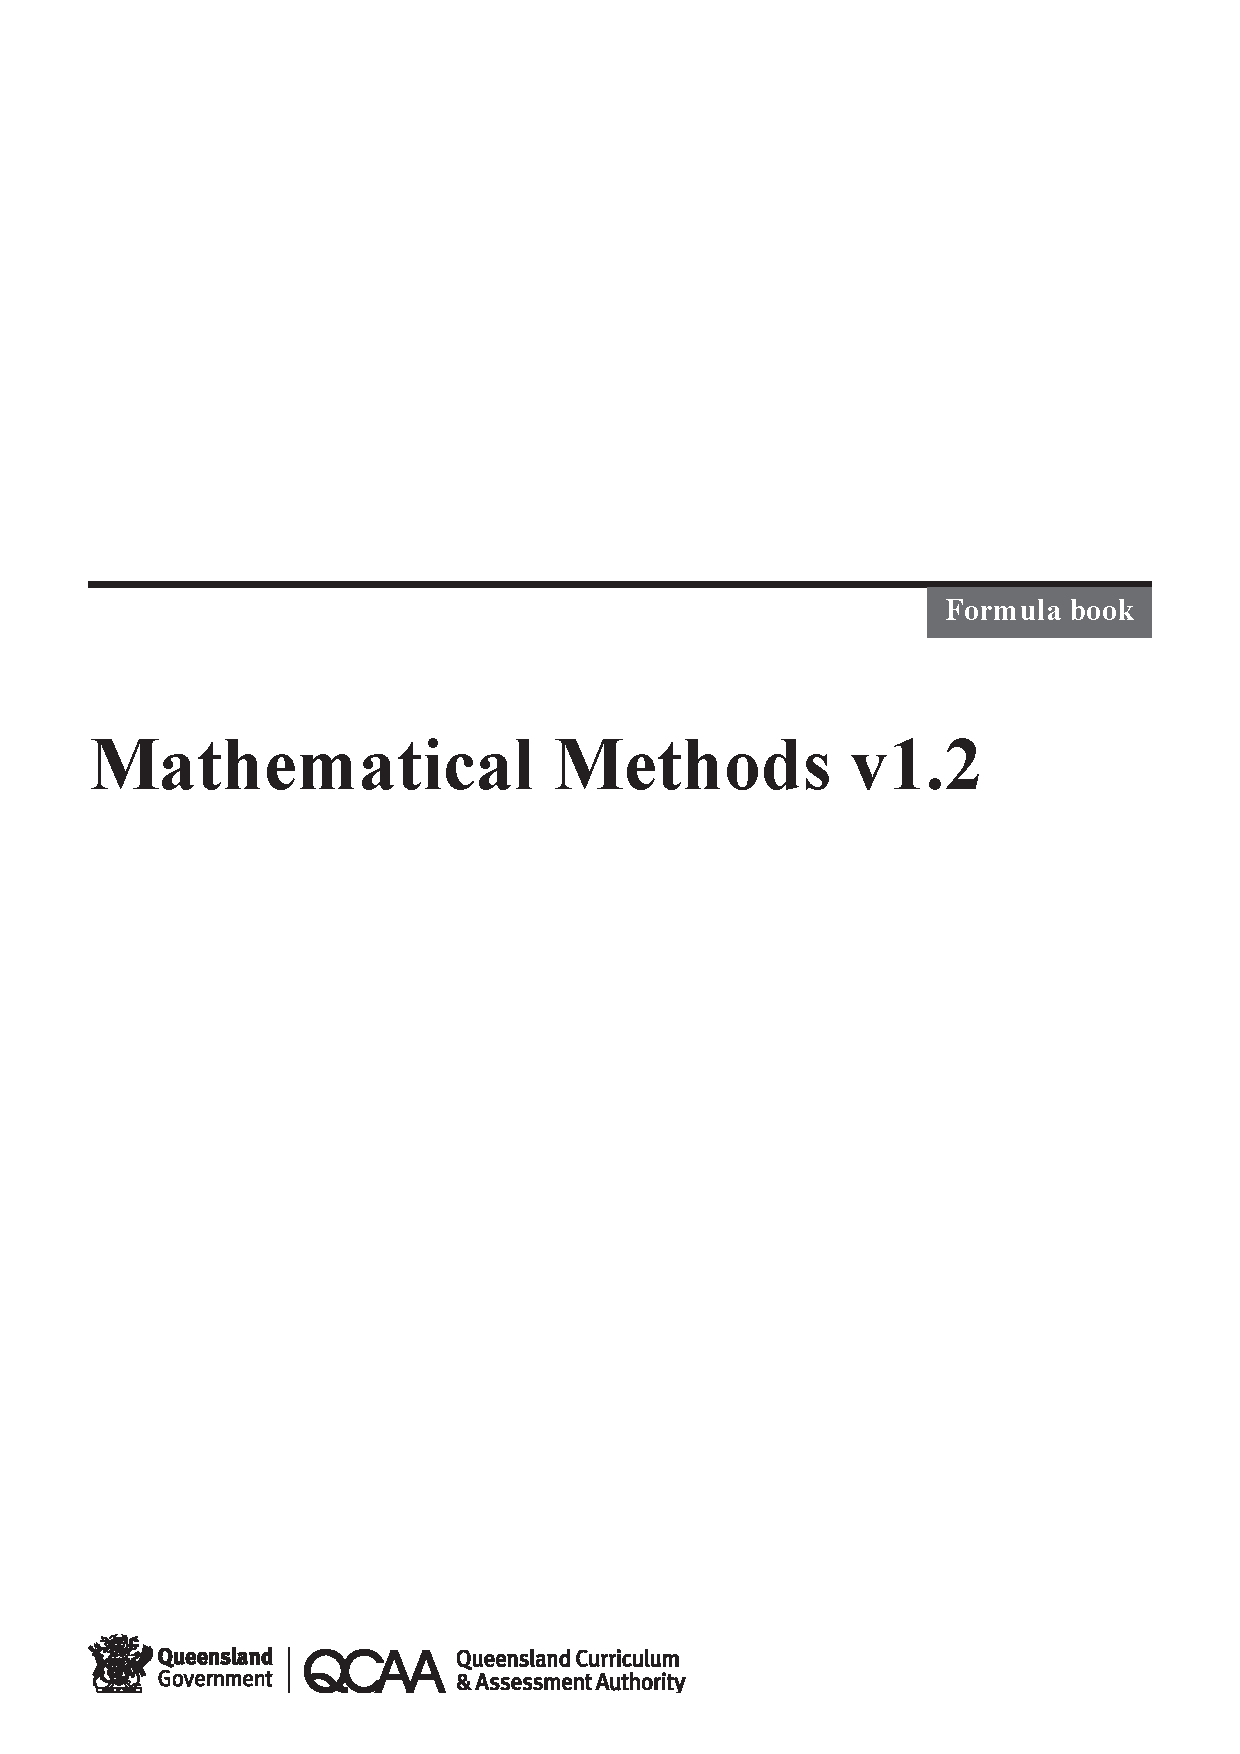
\includepdf[pages=-]{./images/formula-book.pdf}


%%%%%%%%%%%%%%%%%%%%%%%%%%%%%%%%%%%%%%%%%%%%%%%%%%%%%%%%%%%%%%%%

\chapter{Sequences}
\section{Arithmetic sequences}
\begin{generalInformation}
	An arithmetic sequence is a sequence of numbers where the terms are increasing or decreasing at a constant rate.
\end{generalInformation}


\subsection{Recursive definition}
\begin{generalInformation}
	The recursive definition of an arithmetic sequence is:
\end{generalInformation}

\[
	t_{n + 1} = t_n + d
\]

\begin{explanationOfTerms}
	Where $t_{n + 1}$ is the next term, $t_n$ is the current term, and $d$ is the common difference or ``by how much the sequence goes up by".
\end{explanationOfTerms}

\begin{example}
	Let:

	\[
		d := 3, t_n := 4
	\]

	\begin{align*}
		t_{n + 1} & = t_n + d \\
		t_{n + 1} & = 4 + 3   \\
		t_{n + 1} & = 7       \\
		t_{n + 2} & = 7 + 3   \\
		t_{n + 2} & = 10      \\
	\end{align*}
\end{example}


\subsection{General equation}
\begin{generalInformation}
	The general equation for finding the $n^{\text{th}}$ term of the sequence is:
\end{generalInformation}

\[
	t_n = t_1 + (n - 1)d
\]

\begin{explanationOfTerms}
	Where $t_n$ is the $n^{\text{th}}$ term of the sequence, $t_1$ is the first term of the sequence, and $d$ is the common difference.
\end{explanationOfTerms}

\begin{example}
	Let:

	\[
		d := 2, n := 4, t_1 := 8
	\]

	\begin{align*}
		t_n & = t_1 + (n - 1)d \\
		t_n & = 8 + (4 - 1)2   \\
		t_n & = 8 + (3)2       \\
		    & = 8 + 6          \\
		    & = 14
	\end{align*}
\end{example}


\subsection{Sum of all prior arithmetic sequence}
The sum of all arithmetic sequence is given by:

\[
	S_n = \frac{n}{2}(2t_1 + (n - 1)d) = \frac{n}{2}(t_1 + t_n)
\]

\begin{explanationOfTerms}
	Where $S_n$ is the sum of the prior sequences up to the $n^{\text{th}}$ term, $n$ is the number of sequences, $d$ is the common difference, $t_1$ is the first term, and $t_n$ is the $n^{\text{th}}$ term.
\end{explanationOfTerms}

\begin{example}
	Let:

	\[
		
	\]

\end{example}


\section{Geometric sequences}
Geometric sequences are similar to arithmetic sequences, however, it multiplies instead of add the common difference.


\subsection{Recursive definition}
The recursive definition is:

\[
	t_{n + 1} = r \times t_n
\]

Where $t_{n + 1}$ is the next term, $r$ is the common difference, and $t_n$ is the current term.


\subsection{General equation}
The equation for the $n^{\text{th}}$ term is:

\[
	t_n = t_1 \times r^{n - 1}
\]

Where $r$ is the common ratio, $n$ is the term number, $t_n$ is the $n^{\text{th}}$ term, and $t_1$ is the first term.


\subsection{Sum of $n$ geometric sequence}
The sum of the first $n^{\text{th}}$ terms of a geometric sequence is:

\[
	S_n = t_1 \times \frac{r^n - 1}{r - 1}
\]

Where $S_n$ is the sum up to the $n^{\text{th}}$ sequence, $t_1$ is the first term, and $r$ is the common difference.


\subsection{Sum of all geometric sequence}
And the sum of an infinite geometric sequence is:

\[
	S_{\infty} = \frac{t_1}{1 - r}
\]

Where $S_{\infty}$ is the sum up to infinity, $t_1$ is the first term, and $r$ is the common difference.

\begin{note}
	This equation only provides a non-infinite solution where $-1 < r < 1$.
\end{note}


%%%%%%%%%%%%%%%%%%%%%%%%%%%%%%%%%%%%%%%%%%%%%%%%%%%%%%%%%%%%%%%%


\chapter{Functions and relations}
\section{Functions}
\begin{generalInformation}
	Functions is a mathematical concept where if given an input, it performs some operations, and returns an output.  They have the mathematical notation of $f(x)$ where $f$ can be seen as the name of the function and the values within the parenthesis as inputs to the function.  A function must be defined for it to be used.  A simple function which calculates the y-values along a parabola with the x-coordinates as input could be:
\end{generalInformation}

\[
	M(x) := x^2
\]

\begin{align*}
	M(x) & = x^2   \\
	M(3) & = (3)^2 \\
	M(3) & = 9
\end{align*}

Functions can only give a one-to-one relation or a many-to-one relation since there is a clear defined input and output values with the concept of a function.  To check if a graph is a function a \emph{vertical line test} can be performed:
\begin{center}
	If the graph intersects any vertical line more than once, it cannot be a function, and is instead a relation.
\end{center}
\begin{center}
	This is a function:
	\begin{center}
		\begin{tikzpicture}
			\begin{axis}[
					axis lines = left,
					xlabel = $x$,
					ylabel =  $y$
				]
				\addplot[
					domain = -5:5,
					samples = 100,
					color = blue
				]{7*x^3 - 19*x^2 + 3*x - 2};
			\end{axis}
		\end{tikzpicture}
	\end{center}
\end{center}
\begin{center}
	This is not a function:
	\begin{center}
		\begin{tikzpicture}
			\begin{axis}[
					axis lines = left,
					xlabel = $x$,
					ylabel =  $y$
				]
				\addplot[
					domain = -5:5,
					samples = 100,
					color = red
				]({cos(deg(x))}, {sin(deg(x))});
			\end{axis}
		\end{tikzpicture}
	\end{center}
\end{center}

\section{Interval notation}
Interval notation are used to define the range of a function or a relation.  For example, if given a function where the y-values start at 0 and approach but never reach 1, to define the range of the function, it would be $0 \leq y < 1$.  However, this can be rewritten using interval notation as: [0, 1).  The square bracket meaning that it is $=$, $\geq$, and $\leq$, and the parenthesis meaning that it is $<$, or $>$ where it will never reach the value.\\
\begin{note}
	It is called a ``range" when it is the y-value, and a ``domain" when it is the x-value.
\end{note}

\section{Relations}
There are four types of relations, relations meaning for any x-value, how many valid y-values there are.  The four are: one-to-one, many-to-one, one-to-many, and many-to-many.

The first, (one-to-one) relation means that for any x-values, there is only one y-value.  An example would be a straight line:
\begin{center}
	\[f(x) := 2x + 3\]
	\begin{center}
		\begin{tikzpicture}
			\begin{axis}
				\addplot[
					domain = -5:5,
					samples = 100,
				]{2*x + 3};
			\end{axis}
		\end{tikzpicture}
	\end{center}
\end{center}
The second, (many-to-one) relation means that for any y-values, there are more than one x-value.  An example would be a parabola:
\begin{center}
	\[f(x) := x^2\]
	\begin{center}
		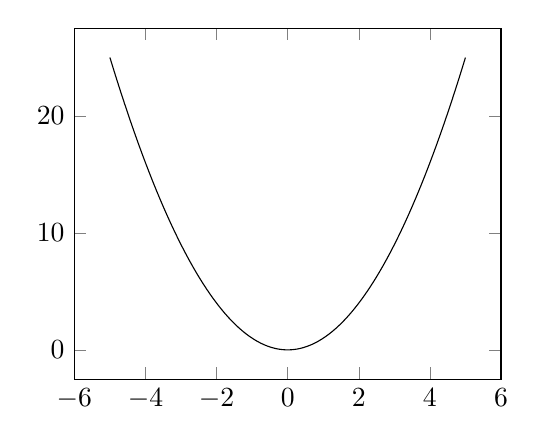
\begin{tikzpicture}
			\begin{axis}
				\addplot[
					domain = -5:5,
					samples = 100,
				]{x^2};
			\end{axis}
		\end{tikzpicture}
	\end{center}
\end{center}
The previous are examples of functions, the next two are not.  The third, (one-to-many) relations means that for any x-value, there are more than one y-value, such as a hyperbola:
\begin{center}
	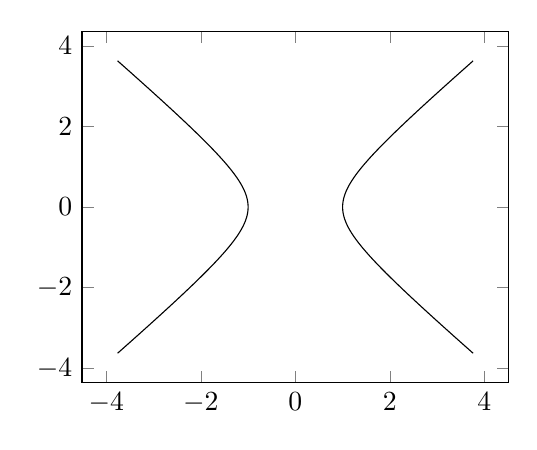
\begin{tikzpicture}
		\begin{axis}
			\addplot [domain=-2:2,samples=100] ({cosh(x)}, {sinh(x)});
			\addplot [domain=-2:2,samples=100] ({-cosh(x)}, {sinh(x)});
		\end{axis}
	\end{tikzpicture}
\end{center}
And for the last, (many-to-many) relations means that for any x-value, there are more than one y-value, and the reverse is also true, such as a circle:
\begin{center}
	\[1 = x^2 + y^2\]
	\begin{center}
		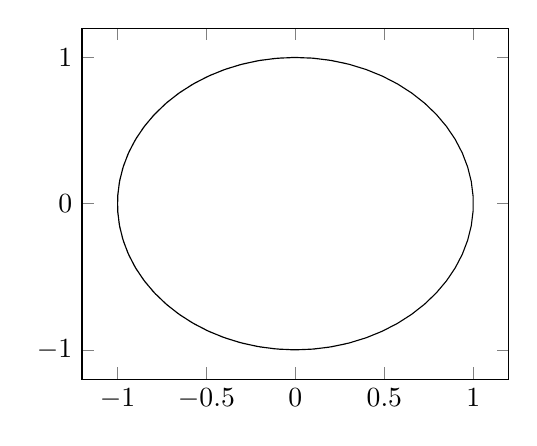
\begin{tikzpicture}
			\begin{axis}
				\addplot[
					domain = -5:5,
					samples = 100,
				]({cos(deg(x))}, {sin(deg(x))});
			\end{axis}
		\end{tikzpicture}
	\end{center}
\end{center}

\chapter{Transformations}
The ways a function can be transformed by some units are:
\[
	y = a \times f(b(x - c)) + d
\]
Where $a$ is the dilation from the x-axis, $b$ is the dilation from the y-axis, $c$ is the translation along the x-axis, and $d$ is the translation along the y-axis.

\section{Dilations}
A dilation transformation means that the function has been either stretched or compressed.  These transformations occur when an output has been multiplied by a dilation factor.  Dilations can either occur in the x-axis or the y-axis.\\
Let y = f(x)\\
When dilated from the x-axis by $a$:
\[
	y = a \times f(x)
\]
When dilated from the y-axis by $b$:
\[
	y = f(x \times b)
\]
\begin{note}
	values less than 1 compresses the function and greater than 1 stretch it
\end{note}

\section{Reflections}
A reflection transformation means that the function has been flipped along an axis.\\
To reflect a function along the x-axis:
\[
	y = -f(x)
\]
To reflect a function along the y-axis:
\[
	y = f(-x)
\]

\section{Translations}
A translation transformation means that the function has been shifted along an axis.\\
To move the function along the x-axis by $c$ units:
\[
	y = f(x - c)
\]
To move the function along the y-axis by $d$ units:
\[
	y = f(x) + d
\]

\chapter{Quadratics}
\section{General or polynomial form}
The general or polynomial form of a quadratic is:
\[
	y = ax^2 + bx + c
\]
\begin{note}
	if $a > 0$ it looks like:
	\begin{center}
		\begin{tikzpicture}
			\begin{axis}[
					axis lines = left,
					xlabel = $x$,
					ylabel = {$f(ax)$},
				]
				\addplot [
					domain=-1:1,
					samples=100,
					color=red,
				] {x^2};
			\end{axis}
		\end{tikzpicture}
	\end{center}
	And $a < 0$ it looks like:
	\begin{center}
		\begin{tikzpicture}
			\begin{axis}[
					axis lines = left,
					xlabel = $x$,
					ylabel = {$f(ax)$},
				]
				\addplot [
					domain=-1:1,
					samples=100,
					color=red,
				] {-(x^2)};
			\end{axis}
		\end{tikzpicture}
	\end{center}
\end{note}
The axis of symmetry or the turning point is found by:
\[
	x = -\frac{b}{2a}
\]

\section{Turning point form}
The turning point form is:
\[
	y = a(x - b)^2 + c
\]
Where $b$ is the translation along the x-axis and $c$ is the translation along the y-axis.

\section{Factorized or x-intercept form}
The factorized or x-intercept form is:
\[
	y = a(x - b)(x - c)
\]
Where it intercepts the x-axis at points $x = b$ and $x = c$

And the axis of symmetry for this form is:
\[
	x = \frac{b + c}{2}
\]

\section{The discriminant}
The discriminant is:
\[
	\Delta = b^2 - 4ac
\]
From a part of the quadratic equation.\\
If $\Delta < 0$, the quadratic has no real factors, $\Delta \geq 0$, the quadratic has 2 real factors, and if $\Delta = 0$, the quadratic is a perfect square and has only 1 real factor.  The number of x-intercepts is equal to the number of factors.

\section{Equations from graphs}
If given the turning point, use the turning point form and substitute the coordinates into $b$ and $c$.  And if given the x-intercepts, use the x-intercept form and substitute the values $b$ and $c$.  While if given 3 points along the curve, use the general form by:\\
\begin{center}
	Given 3 points: $(0, 11), (1, 5), (2, 3)$\\
	Substitute $x$ and $y$ values into general form
	\begin{align*}
		11 & = a(0)^2 + b(0) + c \\
		5  & = a(1)^2 + b(1) + c \\
		3  & = a(2)^2 + b(2) + c
	\end{align*}
	Solve for unknowns
	\begin{align*}
		11 & = \cancelto{0}{a(0)^2} + \cancelto{0}{b(0)} + c   \\
		c  & = 11                                              \\
		5  & = \cancelto{a}{a(1)^2} + \cancelto{b}{b(1)} + c   \\
		5  & = a + b + c                                       \\
		3  & = \cancelto{4a}{a(2)^2} + \cancelto{2b}{b(2)} + c \\
	\end{align*}
	\begin{align*}
		5       & = a + b + 11   \\
		3       & = 4a + 2b + 11 \\
		a + b   & = -6           \\
		4a + 2b & = -8
	\end{align*}
	\begin{align*}
		 & 2 \times (a + b = -6) \\
		 & = -2a + -2b = 12
	\end{align*}
	Using simultaneous equations:
	\begin{align*}
		(4a + 2b     & = -8) \\
		+ (-2a + -2b & = 12) \\
		2a           & = 4   \\
		a            & = 2
	\end{align*}
	\begin{align*}
		2 + b = -6 \\
		b = -8
	\end{align*}
	$\therefore a = 2, b = -8, c = 11$
\end{center}

\section{Solving quadratic equations}
\subsection{Null factor law}
The null factor law means that if $A \times B = 0$ at least $A$ or $B$ must equal 0.
To use the null factor law to calculate the unknowns, factorize the quadratic:
\begin{center}
	If given: $x^2 + 3x - 10 = 0$\\
	$ax^2 + bx + c = $\\
	Find values which add to $b$ and multiply to $c$\\
	$b = 3 = 5 + -2$ and $c = -10 = 5 \times -2$ fit these conditions
	\begin{align*}
		x^2 + 5x + -2x + -10 & = 0     \\
		x(x + 5) + -2(x + 5) & = 0     \\
		(x - 2)(x + 5)       & = 0     \\
		x                    & = 2, -5
	\end{align*}
\end{center}

If the leading coefficient is not 1:
\begin{center}
	\begin{align*}
		2x^2 + 7x + 3 & = 0
	\end{align*}
	find values which multiply to $a \times c$, and add to $b$\\
	$a \times c = 2 \times 3 = 6$, $b = 6 + 1$
	\begin{align*}
		2x^2 + 1x + 6x + 3    & = 0                \\
		x(2x + 1) + 3(2x + 1) & = 0                \\
		(x + 3)(2x + 1)       & = 0                \\
		x                     & = -3, -\frac{1}{2}
	\end{align*}
\end{center}

\subsection{Quadratic equation}
To solve using the quadratic equation, substitute $a$, $b$, and $c$ of the general form into the equation:
\[
	x = \frac{-b \pm \sqrt{b^2 - 4ac}}{2a}
\]

\subsection{Completing the square}
To solve using completing the square, rearrange the equation so that it is in the form:
\[
	x^2 - 2ax + a^2 = (x - a)^2
\]
Example:
\begin{center}
	\begin{align*}
		10x^2 - 30x - 8                                                                              & = 0 \\
		\cancelto{5x^2}{\frac{10x^2}{2}} - \cancelto{15x}{\frac{30x}{2}} - \cancelto{4}{\frac{8}{2}} & = 0 \\
		\cancelto{x^2}{\frac{5x^2}{5}} - \cancelto{3x}{\frac{15x}{5}} - \frac{4}{5}                  & = 0 \\
		x^2 - 3x = \frac{4}{5}
	\end{align*}
	Remember: $x^2 - 2ax + a^2$\\
	$a = \frac{-3}{2}$\\
	$a^2 = \frac{9}{4}$ (In case you forgot, $\frac{a}{b} \times \frac{c}{d} = \frac{ac}{bd}$)
	\begin{align*}
		x^2 - 3x + \frac{9}{4} & = \frac{4}{5} + \frac{9}{4}     \\
		x^2 - 3x + \frac{9}{4} & = \frac{16}{20} + \frac{45}{20} \\
		x^2 - 3x + \frac{9}{4} & = \frac{61}{20}
	\end{align*}
	Remember: $(x - a)^2$
	\begin{align*}
		(x - \frac{3}{2})^2 & = \frac{61}{20}                        \\
		x - \frac{3}{2}     & = \pm \sqrt{\frac{61}{20}}             \\
		x                   & = \frac{3}{2} \pm \sqrt{\frac{61}{20}}
	\end{align*}
\end{center}

\chapter{Factorizing}
\section{Perfect squares}
A perfect square follows the formula:
\[
	(a + b)^2 = a^2 + 2ab + b^2
\]
And
\[
	(a - b)^2 = a^2 - 2ab + b^2
\]

\section{Difference of squares}
A difference of squares follows the formula:
\[
	a^2 - b^2 = (a + b)(a - b)
\]

\section{Equations that reduce to quadratic form}
If given: $ax^4 + bx^2 + c = 0$, $x^2$ could be substituted for $u$, therefore: $au^2 + bu + c = 0$ then solve for $u$.

\chapter{Hyperbolas}
The basic equation of a hyperbola is:
\[
	y = \frac{1}{x}
\]

The lines $x = 0$ and $y = 0$ are asymptotes, which is a line that the function will approach but never reach.\\

The general equation of a hyperbola is:
\[
	y = \frac{a}{x - c} + d
\]
Where $c$ is the vertical asymptote, $d$ is the horizontal asymptote, and $a$ is the dilation factor.

\section{Transformations}
\subsection{Dilation}
A dilation transformation of a hyperbola is:
\[
	y = \frac{a}{x}
\]
Where $a$ is the dilation factor.

\subsection{Translations}
To translate the hyperbola in the y-axis:
\[
	y = \frac{1}{x} + d
\]
Where $b$ is the translation along the y-axis.\\

To translate the hyperbola in the x-axis:
\[
	y = \frac{1}{x - c}
\]
Where $c$ is the translation along the x-axis.\\

To reflect the hyperbola it is:
\[
	y = -\frac{1}{x}
\]

\section{Inverse proportion}
An inversely proportional graph follows a hyperbolic relationship and is represented as:
\[
	y = \frac{k}{x}
\]
Where $k$ is the constant of proportionality.

\chapter{Circles}
Circles are a relation as opposed to a function as it fails the vertical line test, and the equation of a circle is:
\[
	(x - a)^2 + (y - b)^2 = r^2
\]
Where $a$ is the x-component of the centre point,  $b$ is the y-component, and $r$ is the radius.\\

The general form of a circle is the expanded from of the above, and is:
\[
	x^2 + y^2 - 2ax - 2by + a^2 + b^2 -r^2 = 0
\]

\chapter{Polynomials}
Polynomials are an algebraic expression with a positive integer power, such as:
\begin{center}
	$2x^2 - 7x + 2$,\\
	$12x^4 + 2x^3 - 16x^2 + x + 8$\\
	or\\
	$3x^3 + 4$
\end{center}
The degree of a polynomial is the highest power, as an example, the above would be a 2\textsuperscript{nd} degree, 4\textsuperscript{th} degree, and 3\textsuperscript{rd} degree polynomials.  The leading term is the term containing the highest power, again: $2x^2$, $12x^4$, and $3x^3$.  And the constant term is the term that does not contain a variable: $2$, $8$, and $4$.  Polynomials are often shown in function notation:
\[
	P(x) := 2x^3 + 5x - 6
\]

\section{Division}
To divide polynomials by hand, use the long division method shown here:
\begin{center}
	\polylongdiv{x^3 - 12x^2 - 42}{x - 3}
\end{center}

% TODO: step by step instuctions

The product of the division would be in the form:
\[
	\frac{\text{dividend}}{\text{divisor}} = \text{quotient} + \frac{\text{remainder}}{\text{divisor}}
\]
As an overview of what the terms mean:
\begin{center}
	\begin{tabular}{c|c}
		Term      & Meaning                                             \\ \hline
		Dividend  & The number being divided                            \\
		Divisor   & Dividing by                                         \\
		Quotient  & How many times the divisor can go into the dividend \\
		Remainder & After you divide, how much is left over
	\end{tabular}
\end{center}

\section{Remainder theorem}
The remainder theorem is:
\begin{center}
	If a polynomial $P(x)$ is divided by $(x - a)$, then the remainder is $P(a)$.\\
	And If a polynomial $P(x)$ is divided by $(ax - b)$, then the remainder is $P(-\frac{b}{a})$.
\end{center}

To derive this theorem, consider:
\begin{center}
	\begin{align*}
		\frac{P(x)}{x - a}                                 & = \text{quotient} + \frac{\text{remainder}}{x - a}                                                                                                       \\
		\cancelto{P(x)}{\frac{P(x)}{x - a} \times (x - a)} & = \cancelto{(x - a) \times \text{quotient}}{\text{quotient} \times (x - a)} + \cancelto{\text{remainder}}{\frac{\text{remainder}}{x - a} \times (x - a)}
	\end{align*}
	If we let $x = a$:
	\begin{align*}
		P(a) & = 0 \times \text{quotient} + \text{remainder} \\
		P(a) & = \text{remainder}
	\end{align*}
\end{center}

\section{Factor theorem}
A factor of a value means that when the dividend is divided by the divisor, if the result does not produce a remainder, the divisor is a factor of the dividend.  As an example:

We know that 4 is a factor of 12 because it divides 12 exactly into 3 with no remainders, likewise, if $\frac{P(x)}{x - a}$ leaves no remainder, it is a factor of the polynomial:
\[
	P(x) = (x - a) \times \text{quotient}
\]
Or:
\begin{center}
	If $P(x)$ is a polynomial and $P(a) = 0$ then $(x - a)$ is a factor of $P(x)$\\
	And if $P(x)$ is a polynomial and $P(-\frac{b}{a}) = 0$ then $(ax - b)$ is a factor of $P(x)$
\end{center}

\section{Factorizing polynomials}
To factorize a polynomial as a product of linear factors using polynomial division, divide the polynomial by the given factor to get a polynomial of a smaller degree, and factorize the quadratic.
\begin{center}
	Let $P(x) = 4x^3 + 19x^2 + 19x + 6$, and a known factor of $(x + 2)$
	\begin{align*}
		\frac{4x^3 + 19x^2 + 19x + 6}{(x + 2)} & = 4x^2 + 11x - 3          \\
		P(x)                                   & = (x + 2)(4x^2 + 11x - 3)
	\end{align*}
	(factorize $4x^2 + 11x - 3$)
	\begin{align*}
		4x^2 + 11x - 3  & = (x + 3)(4x - 1)        \\
		\therefore P(x) & = (x + 2)(x + 3)(4x - 1)
	\end{align*}
\end{center}

\begin{note}
	if there is a missing factor such as: $ax^3 + cx + d$, just insert a $bx^2$ factor with $b = 0$
\end{note}

\chapter{Probabilities}
\section{Terms}
The key terms of probability are:
\begin{center}
	\begin{tabular}{c|p{8cm}}
		Name                        & Meaning                                                                                                                                          \\ \hline
		Trial                       & a result from something happening                                                                                                                \\
		Outcome                     & a result of a trial                                                                                                                              \\
		Sample space: $\mathcal{E}$ & the set of all outcomes: $\mathcal{E}$ = \{1, 2, 3, 4, 5\}                                                                                       \\
		Event                       & an outcome that we are looking for                                                                                                               \\
		Probability                 & the relative frequency of an event from the set of all outcomes.  Probabilities begin at 0 and end at 1, 0 being impossible and 1 being certain.
	\end{tabular}
\end{center}
\begin{note}
	in a deck of cards, there are 52 cards, there are 4 suits of a heart or a diamond (which are red), and clubs and spades (which are black).  These suits all have an ace, 2, 3, 4 ... 10, a jack, a queen, and a king
\end{note}

\section{Venn diagrams}
\begin{center}
	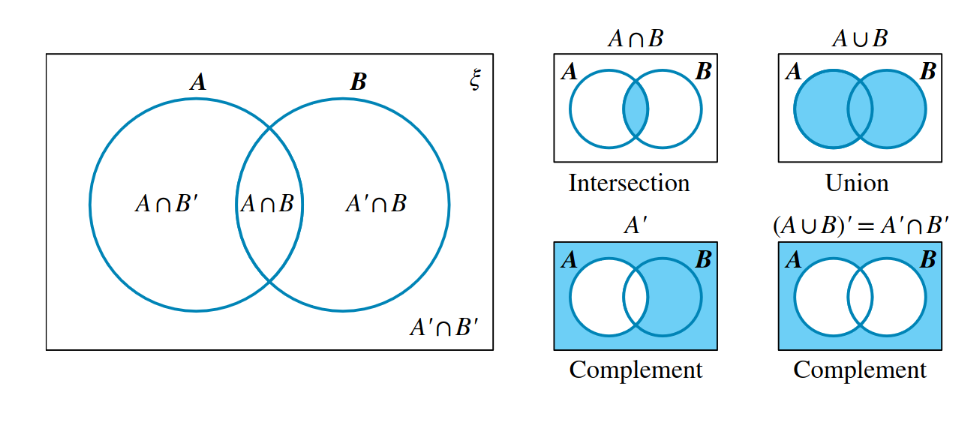
\includegraphics[scale=0.5]{venn diagrams}
\end{center}

\section{Addition}
To add probabilities, use the formula:
\[
	P(A \cup B) = P(A) + P(B) - P(A \cap B)
\]
\begin{note}
	if the events $A$ and $B$ are mutually exclusive, i.e. if $A$ occurs, $B$ cannot possibly happen and vice versa, the addition formula becomes: $P(A \cup B) = P(A) + P(B)$
\end{note}

\section{Probability tables}
Probability tables are a way to represent Venn diagrams in a different format.
\begin{center}
	\begin{tabular}{c|c|c|c}
		    & B              & B'              & sum              \\ \hline
		A   & $P(A \cap B)$  & $P(A \cap B')$  & $P(A)$           \\ \hline
		A'  & $P(A' \cap B)$ & $P(A' \cap B')$ & $P(A')$          \\ \hline
		sum & $P(B)$         & $P(B')$         & $P(\mathcal{E})$
	\end{tabular}
\end{center}

\section{Tree diagrams}
Tree diagrams are used to show the tree of possible outcomes after each trial, as in, if a coin is flipped, it can either be heads or tails, and then a next trial, which could also be heads or tails:
\begin{center}
	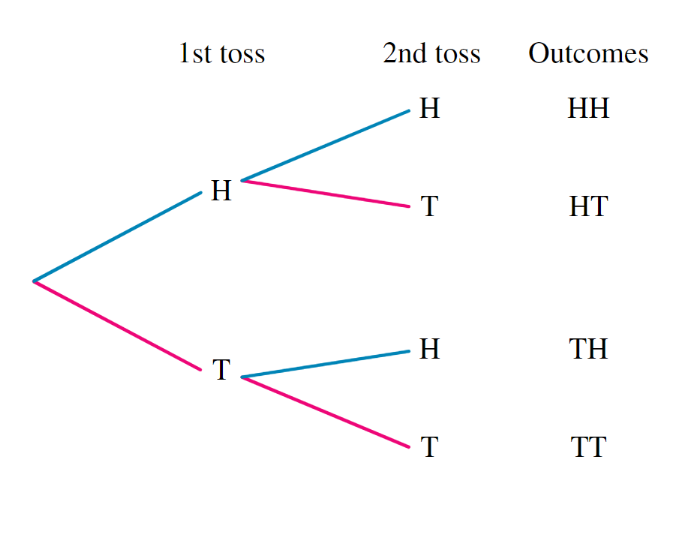
\includegraphics[scale=0.5]{tree diagrams}
\end{center}

Tree diagrams can also be used to calculate probability by multiplying along the branch:
\begin{center}
	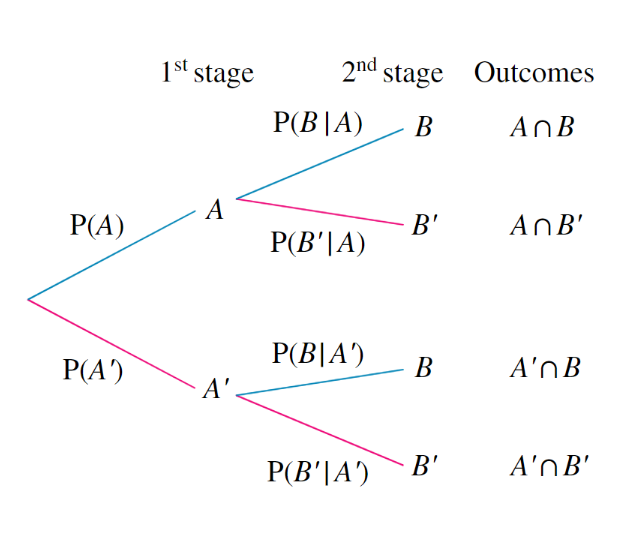
\includegraphics[scale=0.5]{tree diagrams probability}
\end{center}

\section{Conditional probability}
The notation of writing conditional probability is:
\[
	P(A|B)
\]
Where it means that the probability of $A$ given that ($|$) $B$ has occurred.

To calculate the probability of an event, divide the sum of the events occurred over the sum of the sample space:
\[
	P(A) = \frac{n(A)}{n(\mathcal{E})}
\]
And
\[
	P(A \cap B) = \frac{n(A \cap B)}{N(\mathcal{E})}
\]
Similarly, to calculate the probability of an event given another event, change the sum of the sample space to be the sum of the first event:
\begin{align*}
	P(A|B) & = \frac{n(A \cap B)}{n(B)}                                         \\
	       & = n(A \cup B) / n(B)                                               \\
	       & = \frac{n(A \cup B)}{n(\mathcal{E})} / \frac{n(B)}{n(\mathcal{E})} \\
	       & = P(A \cup B) / P(B)                                               \\
	P(A|B) & = \frac{P(A \cap B)}{P(B)}
\end{align*}

\section{Multiplication}
By rearranging the conditional probability formula, the $\cap$ probability formula can be found:
\[
	P(A \cap B) = P(A) \times P(B|A)
\]

\section{Independence}
An independent event is a event which does not change on another event occurring.  Independent events pass these tests:
\begin{align*}
	P(A|B) = P(A) \\
	P(A \cap B) = P(A) \times P(B)
\end{align*}

\section{Addition principle}
If there are $n$ ways of performing operation $A$, and $m$ ways of performing operation $B$, there are $n + m$ ways of performing operation $A \cap B$.

As in, let there be 2 ways to perform task $A$, and 3 ways to perform task $B$.  If there is an option to perform $A$ \emph{or} $B$, there is a total of $2 + 3 = 5$ ways to perform an operation.

\section{Multiplication principle}
If there are $n$ ways of performing operation $A$, and $m$ ways of performing operation $B$, there are $n \times m$ ways of performing operation $A \cup B$.

As in, let there be 4 ways to perform task $A$, and 5 ways to perform task $B$.  With considering 1 way to perform $A$, there are 5 ways to perform $B$, repeat the process through the number of ways to perform $A$.
\begin{center}
	\begin{tabular}{l|lllll}
		       & $B$, 1 & $B$, 2 & $B$, 3 & $B$, 4 & $B$, 5 \\ \hline
		$A$, 1 & (1, 1) & (1, 2) & (1, 3) & (1, 4) & (1, 5) \\
		$A$, 2 & (2, 1) & (2, 2) & (2, 3) & (2, 4) & (2, 5) \\
		$A$, 3 & (3, 1) & (3, 2) & (3, 3) & (3, 4) & (3, 5) \\
		$A$, 4 & (4, 1) & (4, 2) & (4, 3) & (4, 4) & (4, 5) \\
	\end{tabular}
\end{center}
Where there are $4 \times 5 = 20$ ways to perform the operations.

\chapter{Factorials}
Factorials is the result of multiplying all of the integers between the given integer and 1.  This is given the notation and formula:
\[
	n! = n \times (n-1) \times (n-2) \times (n-3)... \times 3 \times 2 \times 1
\]
Example:\\
\begin{align*}
	5! & = 5 \times 4 \times 3 \times 2 \times 1 \\
	   & = 120
\end{align*}

\section{Dividing factorials}
When given some factorial over another factorial in such cases as:
\[\frac{4!}{2!}\]
\[\frac{4 \times 3 \times 2 \times 1}{2 \times 1}\]
\[\frac{4 \times 3 \times \cancel{2 \times 1}}{\cancel{2 \times 1}}\]
\[4 \times 3\]
\[12\]

\section{Special cases}
\[0! = 1\]

\chapter{Permutations}
Permutations is the number of ways of choosing $r$ things from $n$ distinct things where \emph{order matters}.  This is given the notation and formula:
\[
	^nP_r = \frac{n!}{(n-r)!}
\]
Example:
\begin{align*}
	^6P_4 & = \frac{6!}{(6 - 4)!}                                                                 \\
	      & = \frac{6!}{2!}                                                                       \\
	      & = \frac{6 \times 5 \times 4 \times 3 \times 2 \times 1}{2 \times 1}                   \\
	      & = \frac{6 \times 5 \times 4 \times 3 \times \cancel{2 \times 1}}{\cancel{2 \times 1}} \\
	      & = 6 \times 5 \times 4 \times 3                                                        \\
	      & = 360
\end{align*}

\section{Permutations in a circle}
In cases where the positions being concerned is a circle such as the permutations of a circular seating arrangement, if the standard permutations formula is applied, there are several over-counting of the like arrangement in a different perspective.  In these cases apply the formula:
\[
	\frac{^nP_r}{r} = \frac{\frac{n!}{(n-r)!}}{r}
\]

\section{Like objects repetitions}
The number of ways of arranging $n$ objects made up of indistinguishable objects, $n_1$ in the first group, $n_2$ in the second group and so on, is:
\[
	\frac{n!}{n_1! n_2! n_3!... n_r!}
\]
Example:
\begin{center}
	Find the number of permutations of the letters in the world WOOLLOOMOOLOO.\\
	There are 8 'O's and 3 'L's\\
	Permutations:
	\[\frac{13!}{8!3!}\]
	\[\frac{13 \times 12 \times 11 \times 10 \times 9 \times 8 \times 7 \times 6 \times 5 \times 4 \times 3 \times 2 \times 1}{(8 \times 7 \times 6 \times 5 \times 4 \times 3 \times 2 \times 1) \times (3 \times 2 \times 1)}\]
	\[\frac{13 \times 12 \times 11 \times 10 \times 9 \cancel{\times 8 \times 7 \times 6 \times 5 \times 4 \times 3 \times 2 \times 1}}{\cancel{(8 \times 7 \times 6 \times 5 \times 4 \times 3 \times 2 \times 1)} \times (3 \times 2 \times 1)}\]
	\[\frac{13 \times 12 \times 11 \times 10 \times 9}{3 \times 2}\]
	\[\frac{13 \times \cancelto{6 \cancel{\times 2}}{12} \times 11 \times 10 \times \cancelto{3 \cancel{\times 3}}{9}}{\cancel{3 \times 2}}\]
	\[13 \times 6 \times 11 \times 10 \times 3\]
	\[25,740\]
\end{center}

\section{Restrictions}
When considering restrictions, deal with the restrictions first.
Example:
\begin{center}
	Find the number of arrangements of the letters of the word DARWIN beginning and ending with a vowel.
	Number of letters = 6
	Number of positions = 6
	Beginning and end must be a vowel, so the available positions are decreased by 2: number of positions - 2 = 4
	Since 2 vowels must be used:  number of letters - 2 = 4
	Permutations:
	\[^4P_4\]
	\[4!\]
	\[4 \times 3 \times 2 \times 1\]
	\[24\]
\end{center}

\section{Grouped items}
When items are grouped together, treat each group as a single object.  Find the number of arrangements of the groups, then multiply by the number of arrangement within each group.
Example:
\begin{center}
	Find the number of arrangement of the letters of the word EQUALS if the vowels are kept together.
	Number of vowels = 3
	Number of letters = 6
	Number of positions = 6
	As the 3 vowels are grouped together, the number of positions decreases:
	number of positions - 3\textsubscript{for the members of the group} + 1\textsubscript{for the group} = 4
	Permutations within vowel group:
	\[^3P_3 = 3! = 3 \times 2 = 6\]
	Permutations of all positions:
	\[^4P_4 = 4! = 4 \times 3 \times 2 = 24\]
	Multiply together:
	\[6 \times 24 = 144\]
\end{center}

\section{Special cases}
\[^nP_n = n!\]
\[^nP_0 = 1\]

\chapter{Combinations}
Combinations is the number of ways of choosing or selecting $r$ objects from $n$ distinct objects where \emph{order does not matter}.  This is given the notation and formula:
\[^nC_r = \frac{^nP_r}{r!}\]
\[^nC_r = \frac{\frac{n!}{(n-r)!}}{r!}\]
Or
\[
	\binom{n}{r}
\]
Example:
\begin{align*}
	^4C_2 & = \frac{^4P_2}{2!}                                          \\
	      & = \frac{\frac{4!}{(4 - 2)!}}{2!}                            \\
	      & = \frac{\frac{4!}{2!}}{2!}                                  \\
	      & = \frac{\frac{4 \times 3 \times 2}{2}}{2}                   \\
	      & = \frac{\frac{4 \times 3 \cancel{\times 2}}{\cancel{2}}}{2} \\
	      & = \frac{4 \times 3}{2}                                      \\
	      & = \frac{12}{2}                                              \\
	      & = 6                                                         \\
\end{align*}

\section{Pascal's triangle}
The Pascal's triangle is a pattern formed by adding the top 2 adjacent numbers and a 1 is placed on either side of the bottom row to resemble a triangle:
\begin{center}
	\begin{tabular}{rccccccccccccccccccccc}
		$n=0$:  &   &   &    &   &    &    &     &    &     &     & 1                                                     \\\noalign{\smallskip\smallskip}
		$n=1$:  &   &   &    &   &    &    &     &    &     & 1   &     & 1                                               \\\noalign{\smallskip\smallskip}
		$n=2$:  &   &   &    &   &    &    &     &    & 1   &     & 2   &     & 1                                         \\\noalign{\smallskip\smallskip}
		$n=3$:  &   &   &    &   &    &    &     & 1  &     & 3   &     & 3   &     & 1                                   \\\noalign{\smallskip\smallskip}
		$n=4$:  &   &   &    &   &    &    & 1   &    & 4   &     & 6   &     & 4   &    & 1                              \\\noalign{\smallskip\smallskip}
		$n=5$:  &   &   &    &   &    & 1  &     & 5  &     & 10  &     & 10  &     & 5  &     & 1                        \\\noalign{\smallskip\smallskip}
		$n=6$:  &   &   &    &   & 1  &    & 6   &    & 15  &     & 20  &     & 15  &    & 6   &    & 1                   \\\noalign{\smallskip\smallskip}
		$n=7$:  &   &   &    & 1 &    & 7  &     & 21 &     & 35  &     & 35  &     & 21 &     & 7  &    & 1              \\\noalign{\smallskip\smallskip}
		$n=8$:  &   &   & 1  &   & 8  &    & 28  &    & 56  &     & 70  &     & 56  &    & 28  &    & 8  &   & 1          \\\noalign{\smallskip\smallskip}
		$n=9$:  &   & 1 &    & 9 &    & 36 &     & 84 &     & 126 &     & 126 &     & 84 &     & 36 &    & 9 &    & 1     \\\noalign{\smallskip\smallskip}
		$n=10$: & 1 &   & 10 &   & 45 &    & 120 &    & 210 &     & 252 &     & 210 &    & 120 &    & 45 &   & 10 &   & 1 \\\noalign{\smallskip\smallskip}
	\end{tabular}
\end{center}

Each element in the Pascal's triangle can be used to calculate combinations, hence, the triangle can be written using Combinations notation ($^{n}C_r$):
\begin{center}
	\begin{tabular}{rcccccccccccccccc}
		$n=0$: &  &  &  &  &  &         &         &         &         &         & $^0C_0$                                                   \\ \noalign{\smallskip\smallskip}
		$n=1$: &  &  &  &  &  &         &         &         &         & $^1C_0$ &         & $^1C_1$                                         \\ \noalign{\smallskip\smallskip}
		$n=2$: &  &  &  &  &  &         &         &         & $^2C_0$ &         & $^2C_1$ &         & $^2C_2$                               \\ \noalign{\smallskip\smallskip}
		$n=3$: &  &  &  &  &  &         &         & $^3C_0$ &         & $^3C_1$ &         & $^3C_2$ &         & $^3C_3$                     \\ \noalign{\smallskip\smallskip}
		$n=4$: &  &  &  &  &  &         & $^4C_0$ &         & $^4C_1$ &         & $^4C_2$ &         & $^4C_3$ &         & $^4C_4$           \\ \noalign{\smallskip\smallskip}
		$n=5$: &  &  &  &  &  & $^5C_0$ &         & $^5C_1$ &         & $^5C_2$ &         & $^5C_3$ &         & $^5C_4$ &         & $^5C_5$ \\ \noalign{\smallskip\smallskip}
	\end{tabular}
\end{center}

Pascal's triangle shows that the $r^\text{th}$ element of the $n^\text{th}$ row of Pascal's triangle is given by $^nC_r$.  It is assumed that the 1 at the beginning of each row is the $0^\text{th}$ element.  This gives the \emph{Pascal's identity}:
\[^nC_r = ^{n-1}C_{r-1} + ^{n-1}C_r \text{ for } 0 < r < n\]

The Pascal's triangle can be extended to the binomial theorem, where the rule for expanding an expression such as $(a + b)^n$.  Where:
\begin{align*}
	(a + b)^0 & = 1a^0b^0                                                     \\
	(a + b)^1 & = 1a^1b^0 + 1a^0b^1                                           \\
	(a + b)^2 & = 1a^2b^0 + 2a^1b^1 + 1a^0b^2                                 \\
	(a + b)^3 & = 1a^3b^0 + 3a^2b^1 + 3a^1b^2 + 1a^0b^3                       \\
	(a + b)^4 & = 1a^4b^0 + 4a^3b^1 + 6a^2b^2 + 4a^1b^3 + 1a^0b^4             \\
	(a + b)^5 & = 1a^5b^0 + 5a^4b^1 + 10a^3b^2 + 10a^2b^3 + 5a^1b^4 + 1a^0b^5
\end{align*}

\chapter{Index laws}
\begin{center}
	\begin{tabular}{c|c}
		Name                 & Meaning                                             \\ \hline
		Multiplication       & $a^m \times a^n = a^{m + n}$                        \\
		Division             & $\frac{a^m}{a^n} = a^{m - n}$                       \\
		Raising to a power   & $(a^n)^m = a^{n \times m}$                          \\
		To the power of zero & $a^0 = 1$                                           \\
		Negative indices     & $a^{-n} = \frac{1}{a^n}, a \not = 0$                \\
		Fractional indices   & $a^{\frac{m}{n}} = (\sqrt[n]{a})^m = \sqrt[n]{a^m}$
	\end{tabular}
\end{center}

\chapter{Exponential functions}
An exponential function increases or decreases at an accelerating rate, they have an asymptote, a line which it approaches but never reach, and intersect the y-axis at point $(0, 1)$.  The general form of an exponential function equation is:
\[
	y = a^x
\]
Where positive $a$ values increases exponentially, and negative $a$ approaches the asymptote as the x-value increases.

\section{Translations}
To translate the exponential function along the x-axis, use the formula:
\[
	y = a^{x - c}
\]
Where $c$ is the translation along the x-axis.

To translate the exponential function along the y-axis, use the formula:
\[
	y = a^x + d
\]
Where $d$ is the translation along the y-axis.

\section{Dilations}
To dilate the exponential function from the x-axis, use the formula:
\[
	y = b \times a^x
\]
Where $b$ is the dilation factor from the y-axis.  This dilation affects the y-intercept, but the asymptote stays at $y = 0$.

To dilate the exponential function from the y-axis, use the formula:
\[
	y = a^{kx}
\]
Where $k$ is the dilation factor from the y-axis.  This dilation affects the steepness of the graph, but does not affect the y-intercept or the asymptote.

\chapter{Logarithms}
A logarithm is defined as:
\[
	(y = a^x) = (x = \log_ay)
\]
\begin{center}
	\begin{tikzpicture}
		\begin{axis}[
				axis lines = center,
				xlabel = $x$,
				ylabel = {$f(x)$},
			]
			\addplot [
				domain=0.01:10,
				samples=100,
				color=red,
			] {log10(x)};
		\end{axis}
	\end{tikzpicture}
\end{center}
Where $y$ is the base numeral, $a$ is the base, and $x$ is the logarithm for $a > 0$ and $a \not = 1$.

\section{Laws}
\begin{center}
	\begin{tabular}{c|c|c}
		Name                     & Rule                                      & Restrictions                        \\ \hline
		Logarithms of a product  & $\log_a(mn) = \log_am + \log_an$          & $[m, n > 0], [a > 0], [a \not = 1]$ \\
		Logarithms of a quotient & $\log_a(\frac{m}{n}) = \log_am - \log_an$ & $[m, n > 0], [a > 0], [a \not = 1]$ \\
		Logarithms of a power    & $\log_am^n = n\log_am$                    & $[m > 0], [a > 0], [a \not = 1]$    \\
		Logarithms of the base   & $\log_aa = 1$                             & $[a > 0], [a \not = 1]$             \\
		Logarithm of one         & $\log_a 1 = 0$                            & $[a > 0], [a \not = 1]$
	\end{tabular}
\end{center}

\section{The change of base theorem}
To change the base, apply the formula:
\[
	\log_{a}{(x)} = \frac{\log_{b}{(x)}}{\log_{b}{(a)}}
\]
As an example:
\begin{align*}
	\log_{5}25 & = \frac{\log_{10}25}{\log_{10}5} = \frac{1.39794}{0.69897} \approx 2 \\
	\log_{2}8  & = \frac{\ln 8}{\ln 2} = \frac{2.07944}{0.69315} \approx 3            \\
	\log_{3}81 & = \frac{\log_{10}81}{\log_{10}3} = \frac{1.90849}{0.47712} \approx 4
\end{align*}

\chapter{Trigonometry}
\section{Radians and Degrees}
Radians and degrees are two units used to measure angles.  One radian is defined as the angle formed when the length of an arc on a circle is equal to the radius of the circle. There are 2$\pi$ radians in a full circle, where $\pi$ is approximately equal to $3.14159$.

Degrees, on the other hand, are based on the idea that a full circle contains $360\degree$. This means that one degree is equal to $\frac{1}{360}$ of a full circle.

\section{Converting between radians and degrees}
To convert between radians and degrees, we can use the following relationships:
\[
	1\rad = \left({\frac{180}{\pi}}\right)\degree
\]
and
\[
	1\degree = \left(\frac{\pi}{180}\right)\rad
\]

To convert $45\degree$ to radians, use the second relationship:
\begin{align*}
	45\degree & = 45 \cdot \left(\frac{\pi}{180}\right)\rad \\
	          & = \frac{1}{4}\pi\rad
\end{align*}
To convert $\frac{1}{3}\pi$ radians to degrees, use the first relationship:
\begin{align*}
	\frac{1}{3}\pi\rad & = \frac{1}{3}\pi \cdot \left(\frac{180}{\pi}\right)\degree \\
	                   & = 60\degree
\end{align*}

\section{The unit circle}
The unit circle is a circle with the centre point at origin, and has a radius of 1, meaning that it has an equation of $x^2 + y^2 = 1$:
\begin{center}
	\begin{tikzpicture}
		\begin{axis}[
				axis lines=middle,
				axis equal,
				xmin=-1.5, xmax=1.5,
				ymin=-1.5, ymax=1.5,
			]
			\addplot [domain=0:2*pi, samples=100, smooth] ({cos(deg(x))},{sin(deg(x))});
		\end{axis}
	\end{tikzpicture}
\end{center}

\section{Quadrants}
The four sections of a circle is separated into quadrants, the top right being the first quadrant, the top left being the second, the bottom left being the third, and the bottom right being the fourth.
\begin{center}
	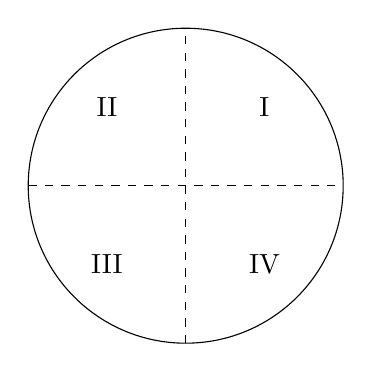
\begin{tikzpicture}
		\draw (0,0) circle (2cm);
		\draw [dashed] (-2,0) -- (2,0);
		\draw [dashed] (0,-2) -- (0,2);
		\node at (1,1) {I};
		\node at (-1,1) {II};
		\node at (-1,-1) {III};
		\node at (1,-1) {IV};
	\end{tikzpicture}
\end{center}
In the first quadrant, the value of all trigonometric functions are positive, however, in the second quadrant, only the sine is, and in the third, only the tangent, and in the forth, only the cosine.
\begin{center}
	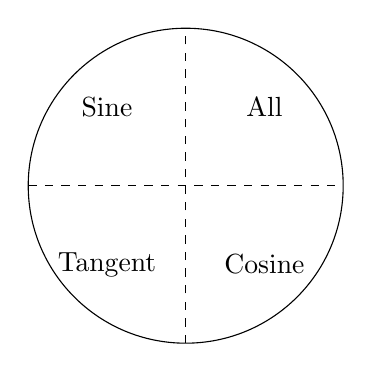
\begin{tikzpicture}
		\draw (0,0) circle (2cm);
		\draw [dashed] (-2,0) -- (2,0);
		\draw [dashed] (0,-2) -- (0,2);
		\node at (1,1) {All};
		\node at (-1,1) {Sine};
		\node at (-1,-1) {Tangent};
		\node at (1,-1) {Cosine};
	\end{tikzpicture}
\end{center}
This is true as sine is the y-axis value of the point along the unit circle which is intersected by an angle, cosine is the x-axis, and tangent is the gradient from the origin to the intersection point.
\begin{center}
	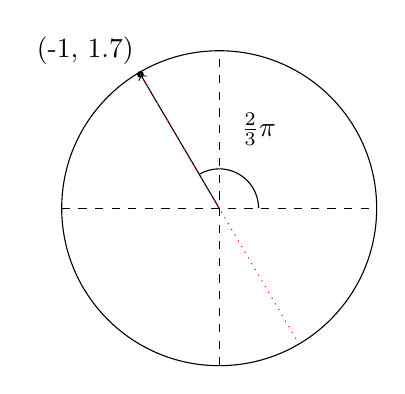
\begin{tikzpicture}
		\draw (0,0) circle (2cm);
		\draw [->] (0,0) -- (-1, 1.7);
		\draw [dashed] (-2,0) -- (2,0);
		\draw [dashed] (0,-2) -- (0,2);
		\node at (-1.7, 2) {(-1, 1.7)};
		\filldraw [black] (-1, 1.7) circle (1pt);
		\draw (0.5, 0) arc (0:120:0.5);
		\node at (0.5, 1) {$\frac{2}{3}\pi$};
		\draw [dotted, red] (-1, 1.7) -- (1, -1.7);
	\end{tikzpicture}
	\begin{align*}
		\therefore \sin\left(\frac{2}{3}\pi\right) & = 1.7            \\
		\cos\left(\frac{2}{3}\pi\right)            & = -1             \\
		\tan\left(\frac{2}{3}\pi\right)            & = \frac{1.7}{-1} \\
		                                           & = -1.7
	\end{align*}
\end{center}

\section{Exact values}
The exact values are as follows:
\begin{center}
	\begin{tabular}{c|c|c|c|c}
		\multicolumn{2}{c|}{Angles ($\theta$)}   & \multicolumn{1}{c|}{\multirow{2}{*}{sin($\theta$)}} & \multicolumn{1}{c|}{\multirow{2}{*}{cos($\theta$)}} & \multicolumn{1}{c}{\multirow{2}{*}{tan($\theta$)}}                         \\
		\multicolumn{1}{l|}{Degrees ($\degree$)} & Radians ($^c$)                                      & \multicolumn{1}{c|}{}                               & \multicolumn{1}{c|}{}                              & \multicolumn{1}{c}{}  \\
		\hline
		0                                        & \multicolumn{1}{c|}{0}                              & \multicolumn{1}{c|}{0}                              & \multicolumn{1}{c|}{1}                             & \multicolumn{1}{c}{0} \\
		\hline
		30                                       & $\frac{1}{6}\pi$                                    & $\frac{1}{2}$                                       & $\frac{\sqrt{3}}{2}$                               & $\frac{1}{\sqrt{3}}$  \\
		\hline
		45                                       & $\frac{1}{4}\pi$                                    & $\frac{1}{\sqrt{2}}$                                & $\frac{1}{\sqrt{2}}$                               & \multicolumn{1}{c}{1} \\
		\hline
		60                                       & $\frac{1}{3}\pi$                                    & $\frac{\sqrt{3}}{2}$                                & $\frac{1}{2}$                                      & $\sqrt{3}$            \\
		\hline
		90                                       & $\frac{1}{2}\pi$                                    & \multicolumn{1}{c|}{1}                              & \multicolumn{1}{c|}{0}                             & n.a.
	\end{tabular}
\end{center}

\section{Graphs}
\subsection{Sine}
\begin{center}
	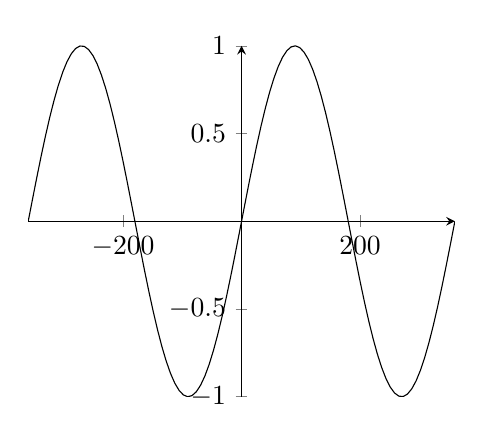
\begin{tikzpicture}
		\begin{axis}[
				axis lines = center
			]
			\addplot[domain=-360:360,samples=100]{sin(x)};
		\end{axis}
	\end{tikzpicture}
\end{center}

\subsection{Cosine}
\begin{center}
	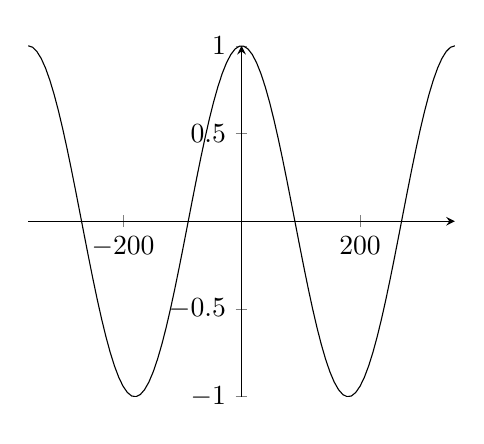
\begin{tikzpicture}
		\begin{axis}[
				axis lines = center
			]
			\addplot[domain=-360:360,samples=100]{cos(x)};
		\end{axis}
	\end{tikzpicture}
\end{center}

\section{Transformations}
\subsection{Amplitude}
\[
	y = A\sin(x)
\]
Where $A$ is the dilation factor, or the amplitude factor.
\begin{center}
	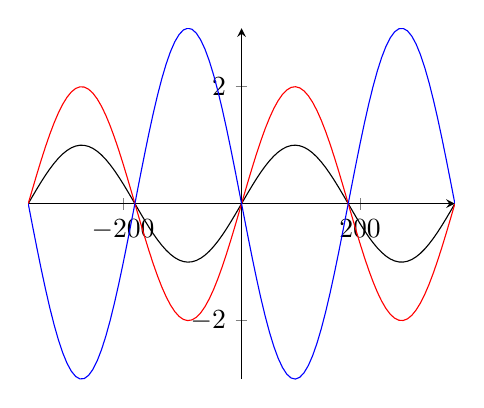
\begin{tikzpicture}
		\begin{axis}[
				axis lines = center
			]
			\addplot[domain=-360:360,samples=100]{sin(x)};
			\addplot[domain=-360:360,samples=100,red]{2 * sin(x)};
			\addplot[domain=-360:360,samples=100,blue]{-3 * sin(x)};
		\end{axis}
	\end{tikzpicture}

	Where the red graph is $2\sin(x)$, black is $\sin(x)$, and blue is $-3\sin(x)$.
\end{center}

\subsection{Period}
\begin{generalInformation}
	To change the length of the wavelength, or the period is as follows:
\end{generalInformation}
\[
	y = \sin(B \times x)
\]
\begin{explanationOfTerms}
	Where $B$ is the dialation from the y-axis or the period.
\end{explanationOfTerms}

\subsection{Equilibrium}

\subsection{Phase}

\chapter{Derivatives}
\section{Rate of change}
\subsection{Constant}

\subsection{Average}

\subsection{Instantanious}

\section{Limits}

\section{First principles}

\section{Derivatives}

\subsection{Velocity and acceleration}

\subsection{Stationary points}

\subsection{Product rule}

\subsection{Chain rule}

\subsection{Quotient rule}

\subsection{Power rule}

\chapter{Probability distributions}
\section{Variables}

\section{Calculating probability distributions}

\section{Expected values}

\section{Standard distribution}

\section{Variance}

\end{document}
